\documentclass[border=6pt]{standalone}
\usepackage{tikz}
\usetikzlibrary{arrows.meta,automata,positioning}
\begin{document}
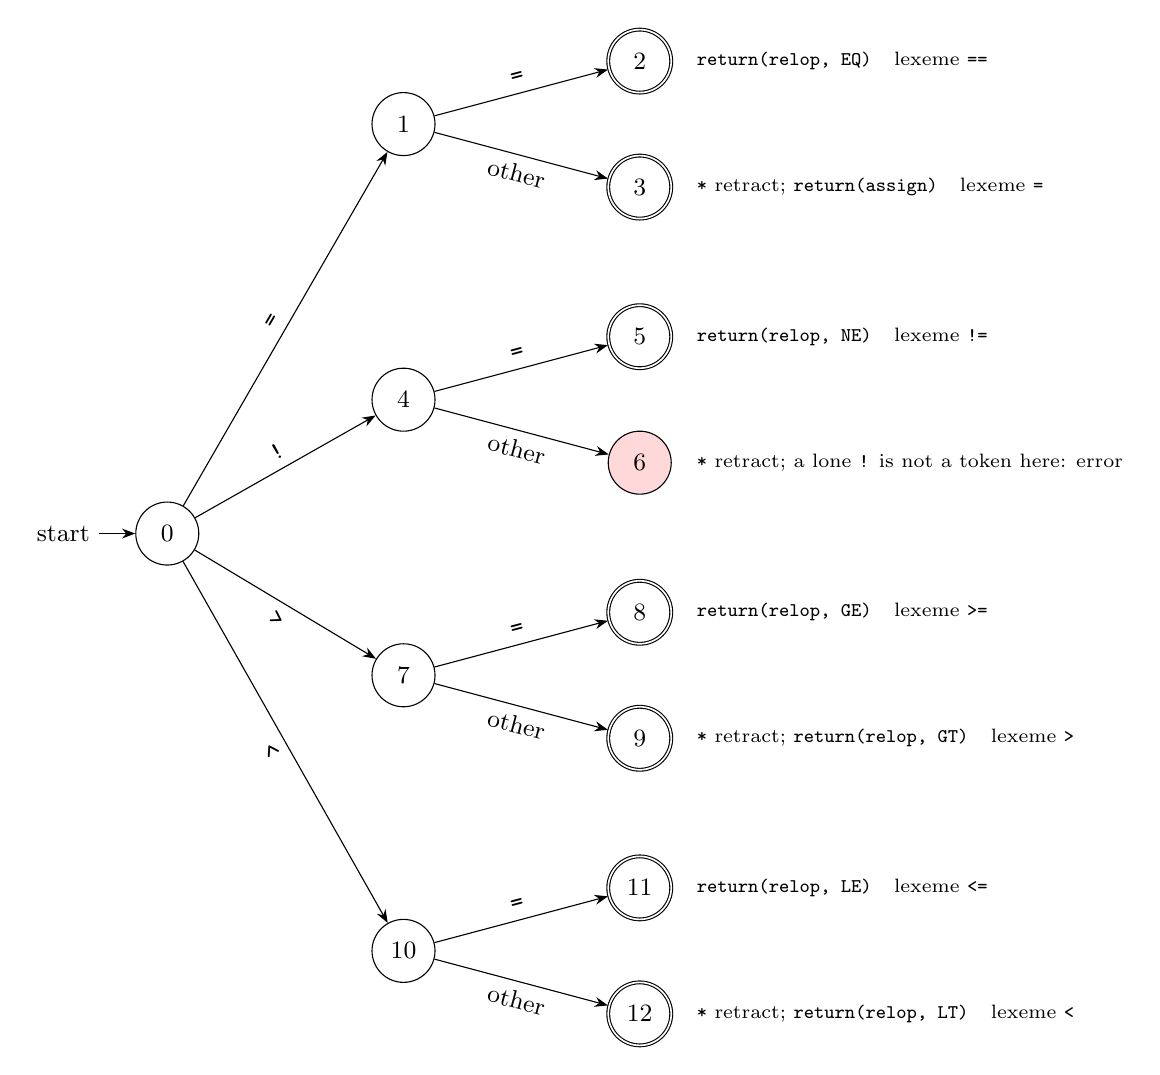
\begin{tikzpicture}[>=Stealth,font=\small,auto,
 every state/.style={minimum size=0.8cm,inner sep=1pt},
 res/.style={font=\scriptsize,anchor=west}]
\node[state,initial] (s0) at (0,0) {0};
% '=' branch
\node[state] (s1) at (3,5.2) {1};
\node[state,accepting] (s2) at (6,6.0) {2};
\node[state,accepting] (s3) at (6,4.4) {3};
\node[res] at (6.6,6.0) {\texttt{return(relop, EQ)}  \ \ lexeme \texttt{==}};
\node[res] at (6.6,4.4) {\texttt{*}  retract; \texttt{return(assign)}  \ \ lexeme \texttt{=}};
% '!' branch
\node[state] (s4) at (3,1.7) {4};
\node[state,accepting] (s5) at (6,2.5) {5};
\node[state,fill=red!15] (s6) at (6,0.9) {6};
\node[res] at (6.6,2.5) {\texttt{return(relop, NE)}  \ \ lexeme \texttt{!=}};
\node[res] at (6.6,0.9) {\texttt{*}  retract; a lone \texttt{!} is not a token here: error};
% '>' branch
\node[state] (s7) at (3,-1.8) {7};
\node[state,accepting] (s8) at (6,-1.0) {8};
\node[state,accepting] (s9) at (6,-2.6) {9};
\node[res] at (6.6,-1.0) {\texttt{return(relop, GE)}  \ \ lexeme \texttt{>=}};
\node[res] at (6.6,-2.6) {\texttt{*}  retract; \texttt{return(relop, GT)}  \ \ lexeme \texttt{>}};
% '<' branch
\node[state] (s10) at (3,-5.3) {10};
\node[state,accepting] (s11) at (6,-4.5) {11};
\node[state,accepting] (s12) at (6,-6.1) {12};
\node[res] at (6.6,-4.5) {\texttt{return(relop, LE)}  \ \ lexeme \texttt{<=}};
\node[res] at (6.6,-6.1) {\texttt{*}  retract; \texttt{return(relop, LT)}  \ \ lexeme \texttt{<}};
\path[->]
 (s0) edge node[above,sloped] {\texttt{=}} (s1)
 (s0) edge node[above,sloped] {\texttt{!}} (s4)
 (s0) edge node[below,sloped] {\texttt{>}} (s7)
 (s0) edge node[below,sloped] {\texttt{<}} (s10)
 (s1) edge node[above,sloped] {\texttt{=}} (s2)
 (s1) edge node[below,sloped] {other} (s3)
 (s4) edge node[above,sloped] {\texttt{=}} (s5)
 (s4) edge node[below,sloped] {other} (s6)
 (s7) edge node[above,sloped] {\texttt{=}} (s8)
 (s7) edge node[below,sloped] {other} (s9)
 (s10) edge node[above,sloped] {\texttt{=}} (s11)
 (s10) edge node[below,sloped] {other} (s12);
\end{tikzpicture}
\end{document}
